% post mortem

\section{Appendix C: Post Mortem}

% \subsection{Our Proposal VS Our Actual Work}
% \label{subsec:our-proposal-vs-our-actual}


\subsection{What Went Well}
The team largely feels that the project went smoothly. The replication was completed successfully, and the team gelled well and operated without conflicts.

\subsubsection{\textbf{We intentionally and carefully designed procedures for effectively producing code, and stuck to them throughout our project.}} At the start of the project, our team clearly laid out procedures for checking code into Git, writing unit tests, conducting code reviews, and communicating with Teams. We established an automated Kanban board and issue tracker, and we maintained a steady backlog of tasks to draw from.

\subsubsection{\textbf{We planned for success!}} We spent a considerable amount of time identifying tasks from the original DeepBugs paper. By conducting a comprehensive review of the process followed by the authors, we were able to identify the major milestones necessary for completing the project. The team went on to further break down each of the milestones into a list of actionable items which would ultimately become the backlog the team used to plan out the replication. This allowed the development process to move along smoothly. During our weekly check-in meetings the team would view the board with this list and easily understand what was in progress and what the next steps were once tasks were completed.

\begin{figure}[h]
    \centering
    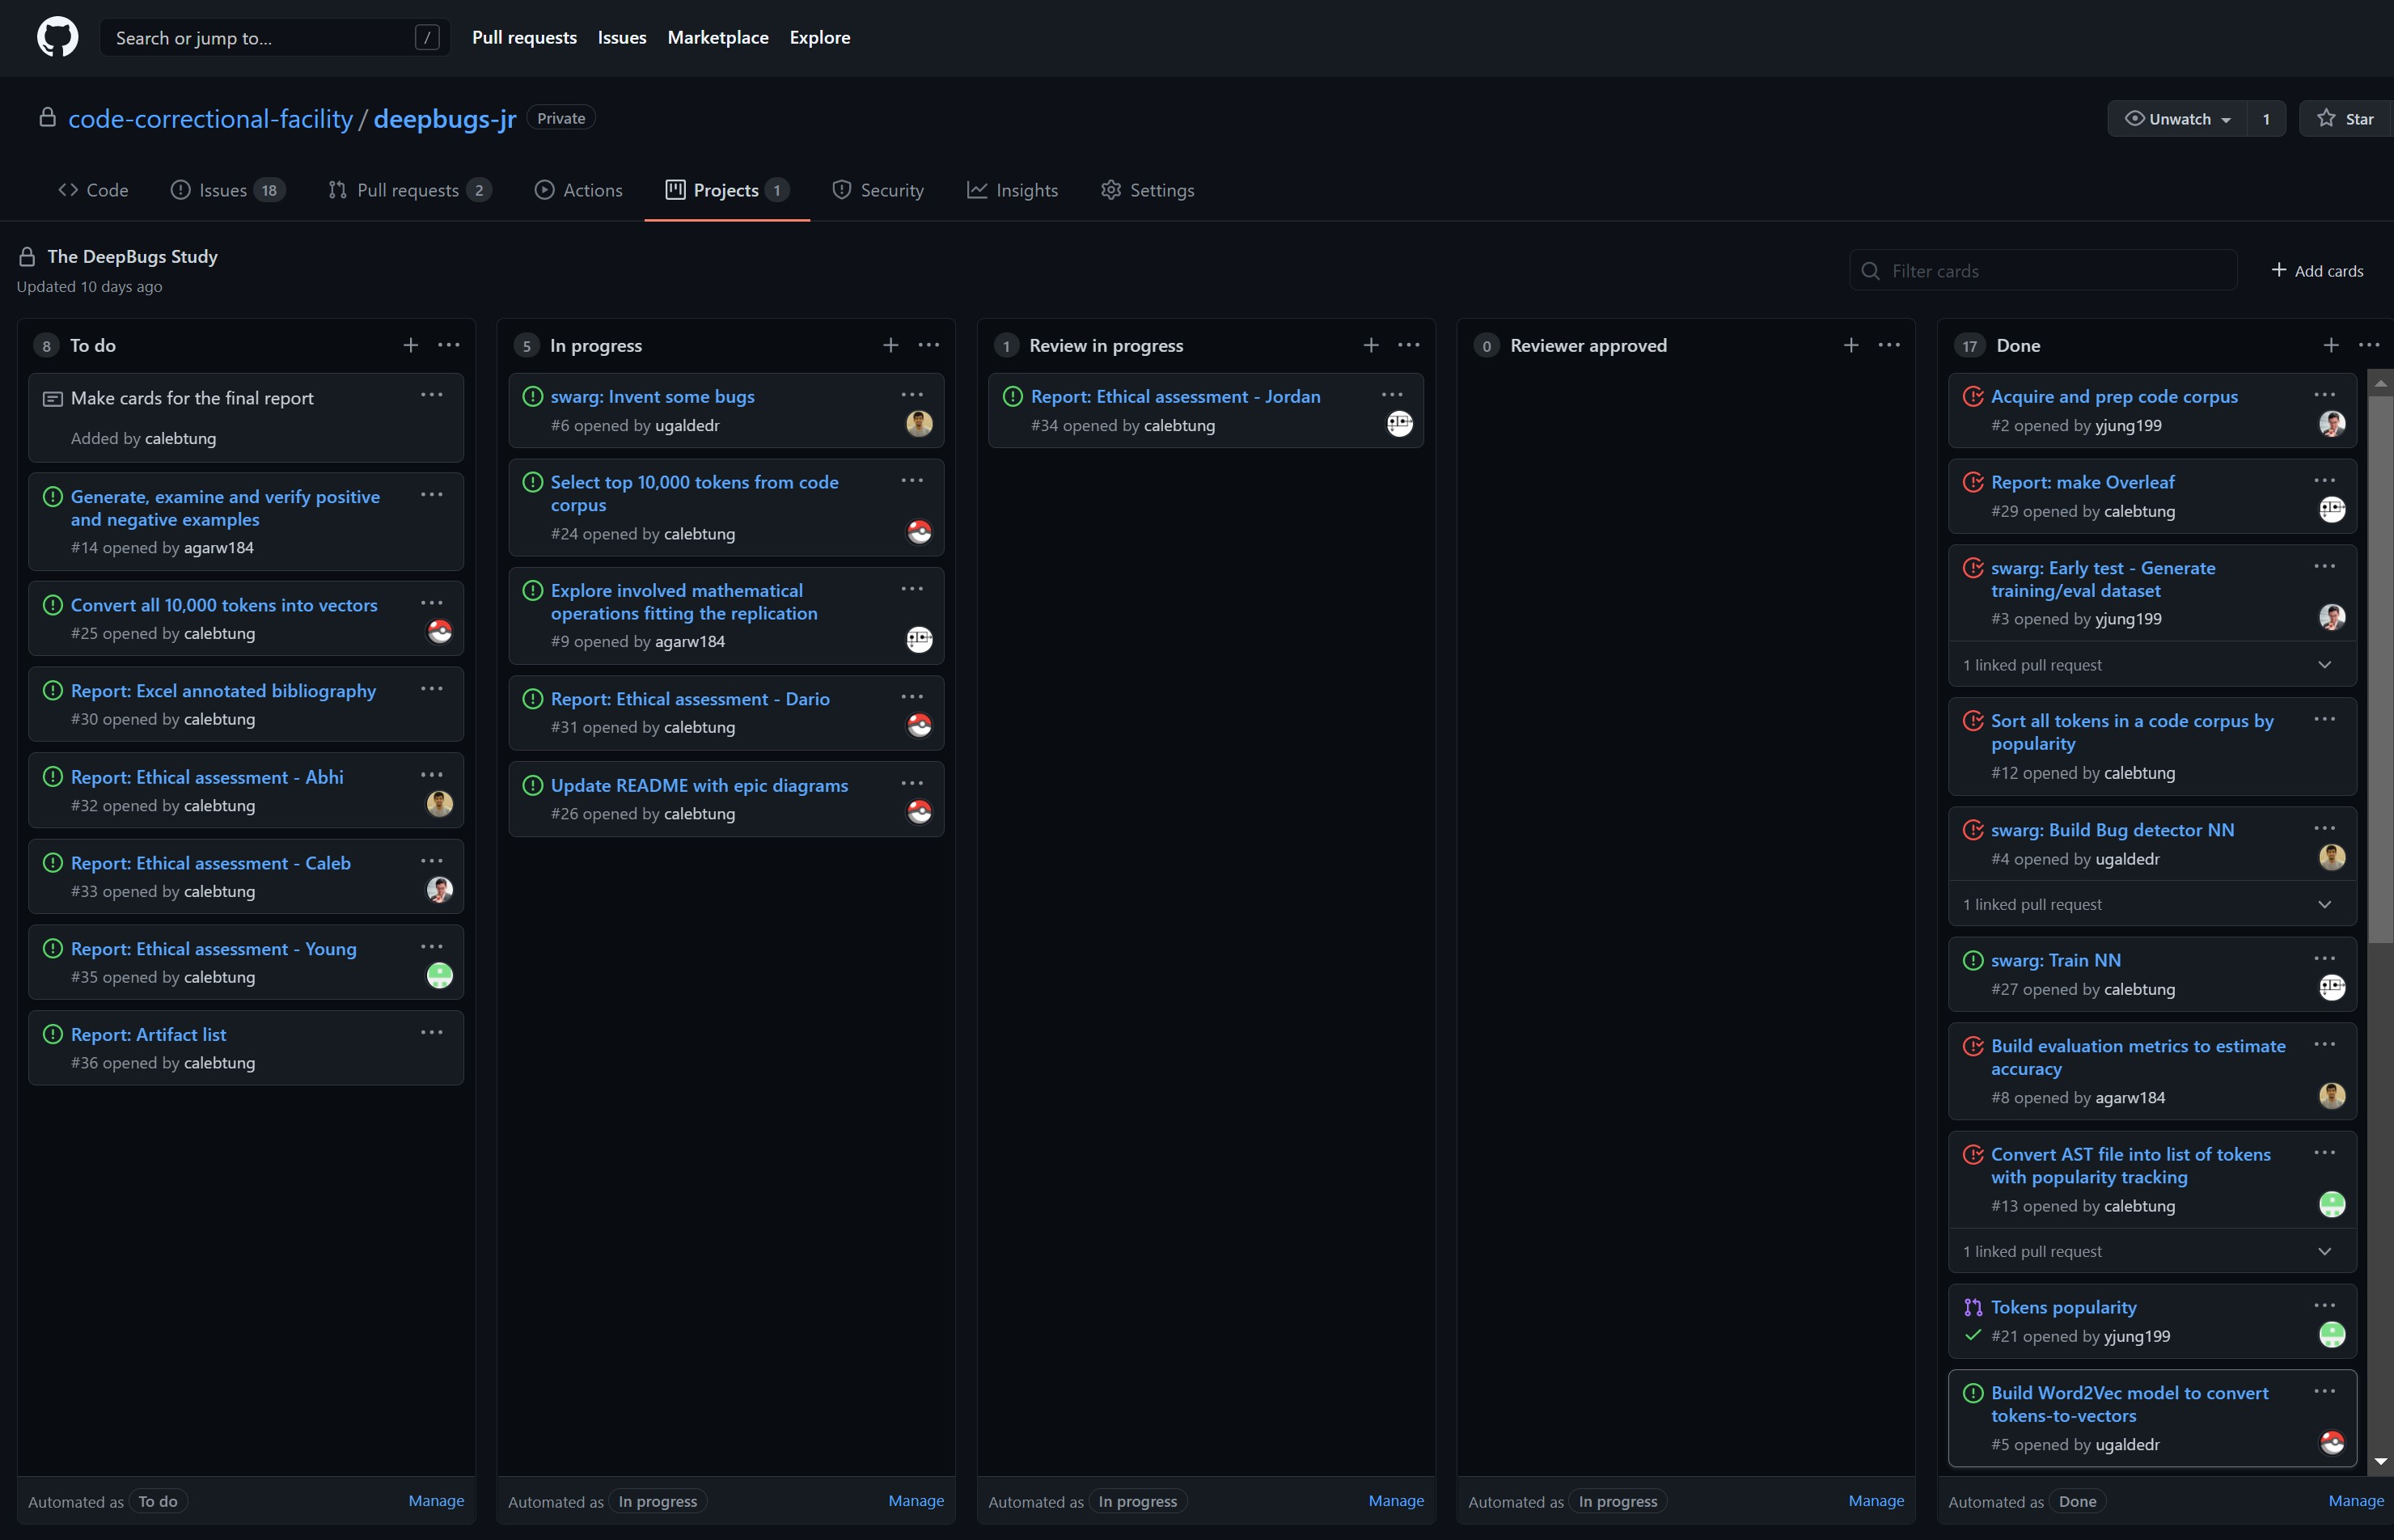
\includegraphics[width=\linewidth]{images/GitHub Projects.jpg}
    \caption{Example of our kanban board with automated issue tracking. As we completed pull requests, the cards automatically rearranged themselves on the board.}
    \label{fig:github-projects}
\end{figure}

\subsubsection{\textbf{Our team collaborated productively.}} Several tasks on the backlog were completed by multiple members working closely together. Although we were careful to assign tasks in bite-sized chunks to stay quasi-Agile, some tasks wound up requiring more assignees. Team members would help each other by pair programming and recommending additional resources. The team did an excellent job of keeping each other in the loop when faced with any issues. This was accomplished by using Microsoft Teams as a general chat. Members would regularly ping the rest of team to ask for advice or alert others on the completion of tasks. The members were highly responsive and received feedback within a matter of minutes in most cases. We all performed manual code reviews to stay familiar with our codebase and ``enforce'' good practices through peer pressure.

\subsubsection{\textbf{We stayed on schedule, with room for flexibility.}} With our team spread across the globe (multiple US timezones and South Korea), we designed our workflow asynchronously, supplemented with regular, synchronous ``tag-up'' meeting times. By investing effort in maintaining a granular, bite-sized backlog, we kept work from getting bottlenecked by members needing to communicate across 13-hour time gaps. US members maintained empty slots in their evening schedules and Korea members kept their mornings open, allowing us to accommodate the few time it was necessary to synchronize outside of meeting time. Our project was thus able to adhere to our schedule, without demanding excessive commitments from team members.

\subsubsection{\textbf{We developed camaraderie.}} No one on the team had met each other prior to the project. By keeping our meetings casual and cracking jokes, the team successfully established a pleasant working environment that was able to complete the project without the usual ``storming'' period of team development.

\subsubsection{\textbf{We produced quality, useful software.}} We created well-documented, test-covered software: an easy-to-use replication of the DeepBugs paper. This would provide more options to users looking to try out the DeepBugs framework (the original authors used mostly JavaScript, but all of our code was written in Python).

\subsubsection{\textbf{We became better engineers.}} Not only was this project a terrific opportunity for us all to gain technical competency in an area of research that we had never dealt with before, but it also allowed us to exercise other software engineering muscles. In order to better understand some of the modern tools used in the software development process, our team set up our Github repository to make use of Github Actions any time code was pushed. This provided members of the team who were not familiar with the typical continuous integration process insight as to how to define and implement a continuous integration pipeline. Building on the development operations process, the python unittest module along with a basic smoke test were implemented to demonstrate a continuous integration pipeline for our project. This allowed members put material discussed earlier in the semester to practical use. We agreed to add tests for branching points to provide coverage as well as, edge cases to ensure proper functionality in the code. In the future, this project could possibly serve as reference material should any team member be required to go through setting up similar infrastructure once again.  


\subsection{What Did Not Go So Well}
Although the project was completed successfully, our team did run into an unanticipated roadblock in the middle of development.


%From SE @ Google: ``A good postmortem should include the following:

%A brief summary of the event

%A timeline of the event, from discovery through investigation to resolution

%The primary cause of the event

%Impact and damage assessment

%A set of action items (with owners) to fix the problem immediately

%A set of action items to prevent the event from happening again

%Lessons learned''

\subsubsection{\textbf{Almost bit off more than we could chew.}} Prior to the project proposal, our team had a very different vision of what our project would look like. Originally, the team had planned to conduct a systemic review on the state-of-art of automated software testing research. In addition to this, the team envisioned the creation of a tool which could direct software engineers to a variety of testing applications intended for the identification of specific bugs. After discussion with Professor Davis following the proposal, the team was reigned in and the scope of the project was narrowed to this replication. It was unfortunate that correcting the team onto this path ate some of the initial planning time leading up to the first status update. In hindsight, now that we've completed our replication, it is quite clear completing a systemic review, generating a tool based on our findings, and compiling this report would not have been feasible within this time frame.

\subsubsection{\textbf{Losing time for 10,000 tokens.}} During the course of development, our team encountered an unnecessary time sink while parsing tokens for training the Word2Vec model. Dario and Young had been assigned tasks to collect the top 10,000 tokens from the source code dataset and train the Word2Vec model. Even after the two spent a week and many precious development hours on the method, the model was still not functioning correctly. After this was brought up during the weekly team meeting, the rest of the team moved to assist, conducting code reviews and familiarizing themselves with the Word2Vec paper. While browsing documentation online, Caleb discovered that the team's desired functionality was actually already implemented in the Word2Vec model framework and could be activated with a single parameter. We wound up discarding the additional code written over the week in favor of this simpler solution. This unfortunate situation could have been avoided by spending a little more time understanding the tools we used for the study. The issue cost the team valuable hours which could have been better spent supporting other tasks. Ultimately, the task was still resolved according to schedule, but any possible time savings were lost. Going forward, scheduling time to do documentation reviews for the tools being used could prevent these types of situations. 
